\documentclass[preview]{standalone}
\usepackage{tikz}
\usepackage{graphicx}
\usetikzlibrary{calc}
\usetikzlibrary{positioning}
\usetikzlibrary{shapes.geometric}
\usetikzlibrary{patterns}
\tikzset{
vertex/.style={circle,draw,black,align=center,inner sep=0cm, minimum size=0.5cm,fill=white,anchor=center},
agent/.style={vertex,fill={rgb:red,1;green,1;blue,1},text=white},
agent1/.style={agent,fill={rgb:red,0;green,1;blue,3}},
agent2/.style={agent,fill={rgb:red,3;green,1;blue,0}},
agent3/.style={agent,fill={rgb:red,1;green,3;blue,2}},
line/.style={black}
}
\begin{document}
\begin{figure}
  \centering
  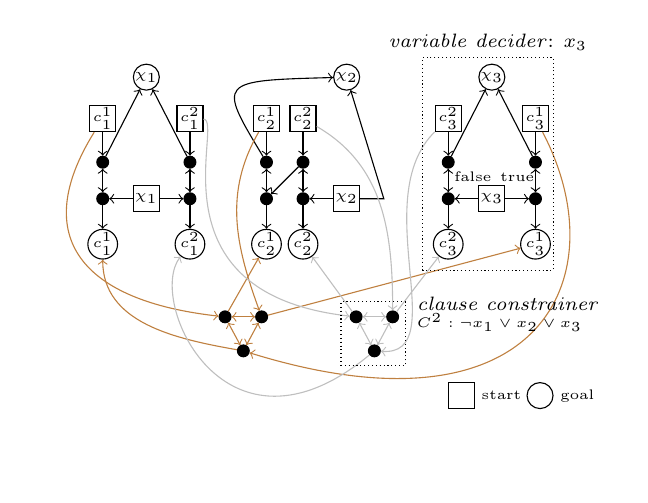
\begin{tikzpicture}
    \newcommand{\edgesize}{0.3cm}
    \newcommand{\edgesizehalf}{0.15cm}
    \newcommand{\edgesizethreetwo}{0.35cm}
    \newcommand{\longedgesize}{1.2cm}
    \tikzset{
      satnode/.style={vertex, minimum size=0.15cm, fill=black},
      start-node/.style={vertex, minimum size=0.33cm,rectangle},
      goal-node/.style={vertex, minimum size=0.33cm},
      line-c1/.style={brown,->},
      line-c2/.style={lightgray,->},
    }
    \tiny
    % x1
    {
      \node[start-node](x1-v1) at (0.0, 0.0) {$\chi_1$};
      %
      \node[satnode, left=\edgesize  of x1-v1](x1-v2) {};
      \node[satnode, right=\edgesize of x1-v1](x1-v3) {};
      %
      \node[goal-node, below=\edgesize of x1-v2](x1-v4) {$c_1^1$};
      \node[goal-node, below=\edgesize of x1-v3](x1-v5) {$c_1^2$};
      %
      \node[satnode, above=\edgesize of x1-v2](x1-v6) {};
      \node[satnode, above=\edgesize of x1-v3](x1-v7) {};
      %
      \node[start-node, above=\edgesize of x1-v6](x1-v8) {$c_1^1$};
      \node[start-node, above=\edgesize of x1-v7](x1-v9) {$c_1^2$};
      %
      \node[goal-node, above=\longedgesize of x1-v1](x1-v10) {$\chi_1$};
      %
      \foreach \u / \v in {v1/v2,v1/v3,v2/v4,v3/v5,v8/v6,v9/v7,v6/v10,v7/v10}
      \draw[line,->] (x1-\u) -- (x1-\v);
      \foreach \u / \v in {v2/v6,v3/v7}
      \draw[line,<->] (x1-\u) -- (x1-\v);
    }
    % x2
    {
      \node[start-node, right=2.2cm of x1-v1](x2-v1) {$\chi_2$};
      %
      \node[satnode,  left=\edgesize of x2-v1](x2-v2) {};
      \node[satnode,  left=\edgesize of x2-v2](x2-v3) {};
      %
      \node[goal-node, below=\edgesize of x2-v2](x2-v4) {$c_2^2$};
      \node[goal-node, below=\edgesize of x2-v3](x2-v5) {$c_2^1$};
      %
      \node[satnode, above=\edgesize of x2-v2](x2-v6) {};
      \node[satnode, above=\edgesize of x2-v3](x2-v7) {};
      %
      \node[start-node, above=\edgesize of x2-v6](x2-v8) {$c_2^2$};
      \node[start-node, above=\edgesize of x2-v7](x2-v9) {$c_2^1$};
      %
      \node[goal-node, above=\longedgesize of x2-v1](x2-v10) {$\chi_2$};
      %
      \foreach \u / \v in {v1/v2,v2/v4,v3/v5,v8/v6,v9/v7,v6/v3}
      \draw[line,->] (x2-\u) -- (x2-\v);
      \coordinate[right=\edgesize of x2-v1](x2-c1);
      \draw[line,->] (x2-v1) -- (x2-c1) -- (x2-v10);
      \foreach \u / \v in {v2/v6,v3/v7}
      \draw[line,<->] (x2-\u) -- (x2-\v);
      \draw[line,->] (x2-v7) .. controls ($(x1-v1)+(0.9, 1.5)$)
      and ($(x1-v1)+(0.9, 1.5)$) .. (x2-v10);
    }
    % x3
    {
      \node[start-node, right=1.5cm of x2-v1](x3-v1) {$\chi_3$};
      %
      \node[satnode,  left=\edgesize of x3-v1](x3-v2) {};
      \node[satnode, right=\edgesize of x3-v1](x3-v3) {};
      %
      \node[goal-node, below=\edgesize of x3-v2](x3-v4) {$c_3^2$};
      \node[goal-node, below=\edgesize of x3-v3](x3-v5) {$c_3^1$};
      %
      \node[satnode, above=\edgesize of x3-v2](x3-v6) {};
      \node[satnode, above=\edgesize of x3-v3](x3-v7) {};
      %
      \node[start-node, above=\edgesize of x3-v6](x3-v8) {$c_3^2$};
      \node[start-node, above=\edgesize of x3-v7](x3-v9) {$c_3^1$};
      %
      \node[goal-node, above=\longedgesize of x3-v1](x3-v10) {$\chi_3$};
      %
      \foreach \u / \v in {v1/v2,v1/v3,v2/v4,v3/v5,v8/v6,v9/v7,v6/v10,v7/v10}
      \draw[line,->] (x3-\u) -- (x3-\v);
      \foreach \u / \v in {v2/v6,v3/v7}
      \draw[line,<->] (x3-\u) -- (x3-\v);
    }
    % c1
    {
      \node[satnode](c1-v1) at ($(x1-v1) + (1.0, -1.5)$) {};
      \node[satnode, right=\edgesize of c1-v1](c1-v2) {};
      \coordinate[right=\edgesizehalf of c1-v1](c1-c1);
      \node[satnode, below=\edgesizethreetwo of c1-c1](c1-v3) {};
      \foreach \u / \v in {v1/v2,v2/v3,v3/v1}
      \draw[line-c1,<->] (c1-\u) -- (c1-\v);
    }
    % c2
    {
      \node[satnode, right=1.5cm of c1-v1](c2-v1) {};
      \node[satnode, right=\edgesize of c2-v1](c2-v2) {};
      \coordinate[right=\edgesizehalf of c2-v1](c2-c1);
      \node[satnode, below=\edgesizethreetwo of c2-c1](c2-v3) {};
      \foreach \u / \v in {v1/v2,v2/v3,v3/v1}
      \draw[line-c2,<->] (c2-\u) -- (c2-\v);
    }
    % lines for c1
    {
      \draw[line-c1](x1-v8) .. controls ($(x1-v1)+(-1.5, -0.5)$)
      and ($(x1-v1)+(-0.8,-1.3)$) .. (c1-v1);
      \draw[line-c1](c1-v3) to[out=170,in=270] (x1-v4);
      \draw[line-c1](x2-v9) to[out=240,in=110] (c1-v2);
      \draw[line-c1](c1-v1) -- (x2-v5);
      \draw[line-c1](x3-v9) .. controls ($(x1-v1)+(6.0,-1.0)$)
      and ($(x1-v1)+(5.0,-3.1)$) .. (c1-v3);
      \draw[line-c1](c1-v2) -- (x3-v5);
    }
    % lines for c2
    {
      \draw[line-c2](x1-v9) .. controls ($(x1-v1)+(1.0, 1.0)$)
      and ($(x1-v1)+(0,-1.2)$) .. (c2-v1);
      \draw[line-c2](c2-v3) .. controls ($(x1-v1)+(1.0, -3.5)$)
      and ($(x1-v1)+(0,-1.3)$) .. (x1-v5);
      \draw[line-c2](x2-v8) to[out=330,in=90] (c2-v2);
      \draw[line-c2](c2-v1) -- (x2-v4);
      \draw[line-c2](x3-v8) .. controls ($(x1-v1)+(2.8, 0.0)$)
      and ($(x1-v1)+(3.9,-2.0)$) .. (c2-v3);
      \draw[line-c2](c2-v2) -- (x3-v4);
    }
    % labels
    {
      \node[start-node, label=right:{start}](label-s) at ($(x1-v1)+(4.0, -2.5)$){};
      \node[goal-node, label=right:{goal}](label-g) at ($(x1-v1)+(5.0, -2.5)$){};
      \node[rectangle,anchor=north west,
      minimum height=2.7cm,text width=1.5cm, draw,densely dotted,
      label=above:{\scriptsize\textit{variable decider}: $x_3$}]
      (box-variable) at ($(x1-v1) + (3.5, 1.8)$) {};
      %
      \node[rectangle,above left=0.2cm of c2-v1,anchor=north west,
      minimum size=0.815cm,draw,densely dotted](box-clause) {};
      \node[anchor=south west](label-clause) at ($(x1-v1)+(3.35,-1.5)$)
      {\scriptsize\textit{clause constrainer}};
      \node[below=0.45cm of label-clause.west, anchor=south west]
      (label-clause-c2) {$C^2: \lnot x_1 \lor x_2 \lor x_3$};
      %
      \node[anchor=south west]
      (label-false) at ($(x3-v2) + (-0.01,0.13)$) {false};
      \node[anchor=south east]
      (label-true) at ($(x3-v3) + (0.07,0.13)$) {true};
    }
  \end{tikzpicture}
\end{figure}
\end{document}
